\section{Introduction}
We have been doing experiments with Iris Plus 3DR\trademark quadricopters in the testing environment of the Smart Mobility Lab of KTH.
The environment is a $5\times5$ meter square area of 2 meters high.
Position of the agents are measured with the motion capture Qualisys\trademark.
The velocity feedback of the quadricopters is running on an offboard computer at 35Hz. The offboard controllers are using the ROS framework.
The computation of the discrete controller is done offline (see digram \ref{diagram}).

\begin{figure}
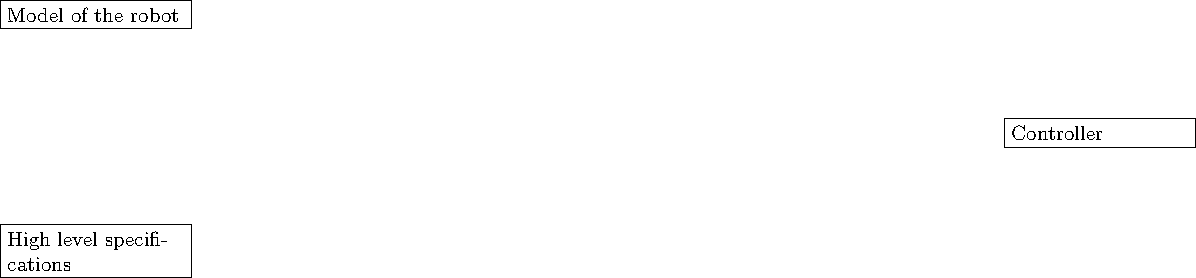
\includegraphics[width=\linewidth]{diagram.tex}
\label{diagram}
\end{figure}

Experiments on single agent, on 1 axis, 2 axis and on multi agents has been done when we managed to find a plan for the model.
The double integrator abstraction (without input memory) leads to abstractions that are unusable in 2D, as the input extended state abstraction with 1 input memory cannot be used with multi agent planning due to size of the abstraction.
